\graphicspath{{content/chapters/2_background/figures/}}

\chapter{Background}%
\label{chp:background}

Existing literature in sports biomechanics highlights the importance of kinematic metrics like stroke length and propulsion symmetry. Computer vision research has successfully applied deep learning for human pose estimation (HPE) and action recognition in water sports. However, a critical limitation in many CV-based swimming systems is the inability to convert pixel movement into absolute, real-world distances, often relying on relative metrics or requiring external sensors.

This project draws upon two key areas of research:
\begin{itemize}
    \item \textbf{Scale Estimation}: Research on using planar objects or known reference markers (fiducial markers) for depth and scale estimation is relevant, which we adapt by using the structured, repetitive nature of the lanerope.
    \item \textbf{Kinematic Segmentation and Symmetry}: Work on segmenting continuous athletic motion (like running or swimming) into discrete phases is essential for calculating time-based metrics (e.g., wall contact time) and assessing symmetry by comparing left and right limb kinematic profiles.
\end{itemize}

\section{Proposed Solution: System Overview}
The proposed system is partitioned into three functional steps: Lanerope Calibration, Feature Extraction, and System Output.

\subsection{Step 1: Lanerope Calibration (Validation Reference)}
This step is the foundation of the system, establishing a stable axis and scale for all downstream measurements. It involves a comparative study of two approaches:
\begin{enumerate}
    \item \textbf{Traditional CV Pipeline}: Utilising colour thresholding (to isolate the coloured floats), edge detection (e.g., Canny), and Hough Transform or RANSAC for line fitting to project a stable reference line along the lanerope's center.
    \item \textbf{CNN-based Pipeline}: Implementing a keypoint detection or semantic segmentation model (e.g., a customised U-Net or Mask R-CNN) to identify the boundary or center points of the lanerope floats. This is expected to offer better robustness against water splash and varying lighting.
\end{enumerate}
The results of these two pipelines will be used to create the Calibration Module, converting pixel-based distances into real-world meters.

\subsection{Step 2: Feature Extraction – Starts, Swim, and Turns}
With the metric scale in place, a robust pose-estimation model will track the swimmer's key joints. A sequence-modelling approach will then segment the footage to extract biomechanical features across the three domains:
\begin{itemize}
    \item \textbf{Starts}: Metrics include reaction time, leap and flight times, underwater speed and distance, and shoulder/arm position at the end of the first pull.
    \item \textbf{Swim (Mid-Pool)}: Focus on stroke length (hand entry to exit in meters) and impulse (distance covered per stroke). This step will also facilitate the left–right symmetry assessment by comparing the angular and linear velocities of the corresponding limbs during the catch and pull phases.
    \item \textbf{Turns}: Metrics include stroke rate before the wall, entry-to-wall contact time, wall contact duration, and push-to-breakout measures (underwater distance and shoulder/arm positions leading to the second stroke).
\end{itemize}

\section{Evaluation Plan}
The evaluation strategy is two-fold, encompassing a rigorous quantitative assessment of the core technology and a qualitative validation of the final derived metrics.

\subsection{Quantitative Evaluation}
\begin{itemize}
    \item \textbf{Lanerope Accuracy Comparison}: The two lanerope pipelines (Traditional CV and CNN) will be assessed against annotated ground truth. Metrics will include axis error (deviation from the true lanerope angle), scale error (difference from the known float interval distance), and frame-to-frame jitter (stability).
    \item \textbf{Downstream Metric Accuracy}: The lanerope method yielding the lowest error will be used to calibrate the system. The final system's metric outputs (e.g., a calculated 5-meter distance) will be compared to a physically measured distance to quantify the final distance estimation accuracy.
\end{itemize}

\subsection{Qualitative Validation}
\begin{itemize}
    \item \textbf{Annotated Footage Comparison}: System outputs (keypoints, trajectories, and phase segmentations) will be overlaid onto the original video and validated against human-annotated samples.
    \item \textbf{Expert Feedback}: Structured interviews and feedback sessions will be conducted with certified swimming coaches to assess the interpretability, practical value, and actionability of the generated performance reports (e.g., symmetry score, wall contact duration).
\end{itemize}

\section{Conclusions including Expected Outcomes and Difficulties/Challenges}
This project is expected to deliver a robust proof-of-concept system capable of providing high-value, objective biomechanical data from standard video. The expected outcomes include the validated optimal lanerope calibration method (Traditional CV or CNN) and a working pipeline that accurately calculates and visualises metrics across Starts, Swim, and Turns.

Key challenges and difficulties anticipated include:
\begin{itemize}
    \item \textbf{Data Annotation}: Obtaining sufficient, high-quality, frame-by-frame annotated footage for training the CNN-based lanerope model and for ground-truthing the pose/phase segmentation.
    \item \textbf{Generalisation}: Ensuring the lanerope calibration method is robust against varying pool environments, lighting conditions, and camera angles (beyond a fixed setup).
    \item \textbf{Symmetry Complexity}: Developing a sufficiently sensitive metric to accurately quantify left–right symmetry, given the inherent small variances in human movement.
\end{itemize}

% % Figure~\ref{fig:sample} shows a sample figure and how to cross-reference
% % figures.
% %
% % \begin{figure}[htbp]
% %     \centering
% %     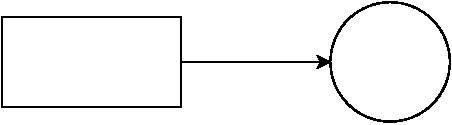
\includegraphics[width=\textwidth,keepaspectratio]{sample}
% %     \caption[Short sample caption.]{Longer caption that  and shows below the figure.\label{fig:sample}}
% % \end{figure}
% %


% \section{Literature Review}%
% \label{sec:literature_review}
% The effective analysis of swimming technique is a complex and crucial aspect of competitive swimming. Traditionally, this process has been performed by coaches who rely on their expertise and visual observation, often supplemented by slow-motion video playback. However, this manual approach is inherently subjective, time-consuming, and may miss subtle biomechanical inefficiencies. The emergence of AI and computer vision offers the potential to provide a more objective and consistent analysis, enabling swimmers and coaches to gain deeper insights into performance.

% This project's wider context is the burgeoning field of sports analytics, where AI is used to optimize training, prevent injuries, and enhance athletic performance across various disciplines. The anticipated benefits of the proposed system include the ability to provide instant, precise feedback on technique, helping swimmers to correct asymmetries and refine their stroke patterns. The likely users of this system are competitive swimmers, their coaches, and sports scientists seeking to research human motion.

% The theoretical foundation of this project lies in the fields of computer vision and machine learning. Specifically, the system will utilize pose estimation, a computer vision task that identifies the location of a person's joints from an image or video. This data is then used in a sequence modeling context to analyze temporal patterns of motion. The software development will utilize a programming language like Python, leveraging common AI libraries such as TensorFlow or PyTorch, and a chosen off-the-shelf pose estimation model.
% \section{Instructions}%
% \label{sec:instructions}

% This sentence refers to Section~\ref{sec:literature_review}, as an example of
% how to do cross-referencing.
% Equation~\eqref{eq:emc} shows one of the most famous equations.
% %
% \begin{equation}
%     \label{eq:emc}
%     e = mc^2
% \end{equation}
% %
% An example of how to create multiple equations, where they all align is given
% below.
% %
% \begin{align}
%     e & = mc^2          \\
%     m & = \frac{e}{c^2}
% \end{align}

% \section{Inserting references}%
% \label{sec:inserting_references}

% To insert a reference, the entry must be inserted in the \texttt{references.bib}
% file.
% The key or unique ID of the entry is then used to refer to it.
% \LaTeX{} will automatically number the entry and generate the list of
% references.
% The paper in~\cite{sample_key} is used as a referencing example.

% \section{Inserting acronyms}%
% \label{sec:inserting_acronyms_and_glossary_entries}

% The \gls{tcp} and \gls{udp} protocols are two layer 4 protocols, used for
% demonstrating how to use acronyms.
% On the second use of an acronym, only its initials are shown as demonstrated in
% the following sentence.
% The \gls{tcp} and \gls{udp} protocols are two layer 4 protocols, used for
% demonstrating how to use acronyms.

% \section{Using glossary terms}%
% \label{sec:using_glossary_terms}

% Let \gls{G} represent a loop-free directed graph, where \gls{V} and \gls{E}
% represent the set of nodes and edges, respectively.

% \section{Inserting a table}%
% \label{sec:inserting_a_table}

% A simple table is shown in Table~\ref{tab:simple}, with a more complex example
% given in Table~\ref{tab:complex}.

% \begin{table}
%     \caption{Simple table example.\label{tab:simple}}
%     \centering
%     \begin{tblr}{|c|S[table-format=3.2]|c|}
%         \hline
%         \textbf{Header 1} & \textbf{Header 2} & \textbf{Header 3} \\
%         \hline
%         1                 & 2.3               & Orange            \\
%         2                 & 100.5             & Blue              \\
%         3                 & 35.0              & Black             \\
%         \hline
%     \end{tblr}
% \end{table}

% \begin{table}
%     \centering
%     \caption{Complex table example.\label{tab:complex}}
%     \begin{tblr}{|Q[m,0.2\textwidth]|Q[m,0.2\textwidth]|Q[m,0.2\textwidth]|Q[m,0.2\textwidth]|}
%         \hline
%         \SetCell[r=2]{c} Table Head & \SetCell[c=3]{c} Table Column Head & & \\
%         \hline
%         & Table column subhead 1 & Table column subhead 2 & Table column subhead 3 \\
%         \hline
%         Item 1 & 2 & 3 & 4 \\
%         \hline
%         Item 2 & 2 & 3 & 4 \\
%         \hline
%         Item 3 & 2 & 3 & 4 \\
%         \hline
%         Item 4 & 2 & 3 & 4 \\
%         \hline
%     \end{tblr}
% \end{table}

% \section{Inserting code snippet}%
% \label{sec:inserting_code_snippet}

% The code snippet in Listing~\ref{lst:python_example} demonstrates a very simple
% python program.

% \begin{lstlisting}[language=Python,caption=Python example,label={lst:python_example}]
% def main() -> None:
%     print("Hello World")

% if __name__ == "__main__":
%     main()
% \end{lstlisting}

% \section{Inserting theorems, corollaries and lemmas}%
% \label{sec:inserting_theorems,_corollaries_and_lemmas}

% \begin{theorem}
%     Let \(f\) be a function whose derivative exists in every point, then \(f\) is
%     a continuous function.
% \end{theorem}

% \begin{theorem}[Pythagorean theorem]
%     \label{pythagorean}
%     This is a theorem about right triangles and can be summarised in the next
%     equation
%     \[ x^2 + y^2 = z^2 \]
% \end{theorem}

% And a consequence of theorem \ref{pythagorean} is the statement in the next
% corollary.

% \begin{corollary}
%     There's no right rectangle whose sides measure 3cm, 4cm, and 6cm.
% \end{corollary}

% You can reference theorems such as \ref{pythagorean} when a label is assigned.

% \begin{lemma}
%     Given two line segments whose lengths are \(a\) and \(b\) respectively there is a
%     real number \(r\) such that \(b=ra\).
% \end{lemma}

% \section{Inserting an algorithm}%
% \label{sec:inserting_an_algorithm}

% The pseudocode for a basic \gls{ea} using NSGA-II is given in
% Algorithm~\ref{alg:evolutionaryAlgorithm}.

% \begin{algorithm}
%     \caption{Pseudocode for an Evolutionary Algorithm}%
%     \label{alg:evolutionaryAlgorithm}
%     \begin{algorithmic}
%         \State \( \mathcal{P} \) = Population Size
%         \State \( \chi \) = Number of Generations
%         \State \( \omega \) = Crossover Probability
%         \State \( \psi \) = Mutation Probability
%         \State
%         \State population = GenerateInitialPopulation(\( \mathcal{P} \))
%         \For{\( 1, 2, \ldots, \chi \)}
%         \State offspring = TournamentSelection(population, \( \mathcal{P} \))
%         % Crossover
%         \For{\(c_i \in \) offspring, \( i = 1, 3, 5, \ldots, \mathcal{P}\)}
%         \State \(z\) = random(0, 1)
%         \If{\( z < \omega \)}
%         \State Crossover(\( c_i, c_{i+1} \))
%         \EndIf
%         \EndFor
%         % Mutation
%         \For{\(c_i \in \) offspring}
%         \State \(z\) = random(0, 1)
%         \If{\( z < \psi \)}
%         \State Mutate(\( c_i \))
%         \EndIf
%         \EndFor
%         % Calculate fitness
%         \State CalculatePopulationFitness(offspring)
%         % Update population size
%         \State population = NSGA-II([population + offspring], \(\mathcal{P}\))
%         \EndFor
%     \end{algorithmic}
% \end{algorithm}
